\chapter{関連研究}
\label{chp:first}

\section{関連研究}
\label{sec:paragraph}
新しいマテリアルを使い,今までにない3Dプリンターでは表現できなかったモノを作ることを可能にしている研究を中心最新の3Dプリンターに関する研究を調査した.


\section{ゲルを用いて印刷する3Dプリンター\cite{a}}
\label{sec:enum}

この研究は,ゲルをマテリアルとして用いた造形物を3Dプリンディングするものである.
図2.1のように,ゲル溶液を使用しながら強度や感触を部位によって変化させて造形物を作成することができる.

\begin{figure}[H]
  \centering
  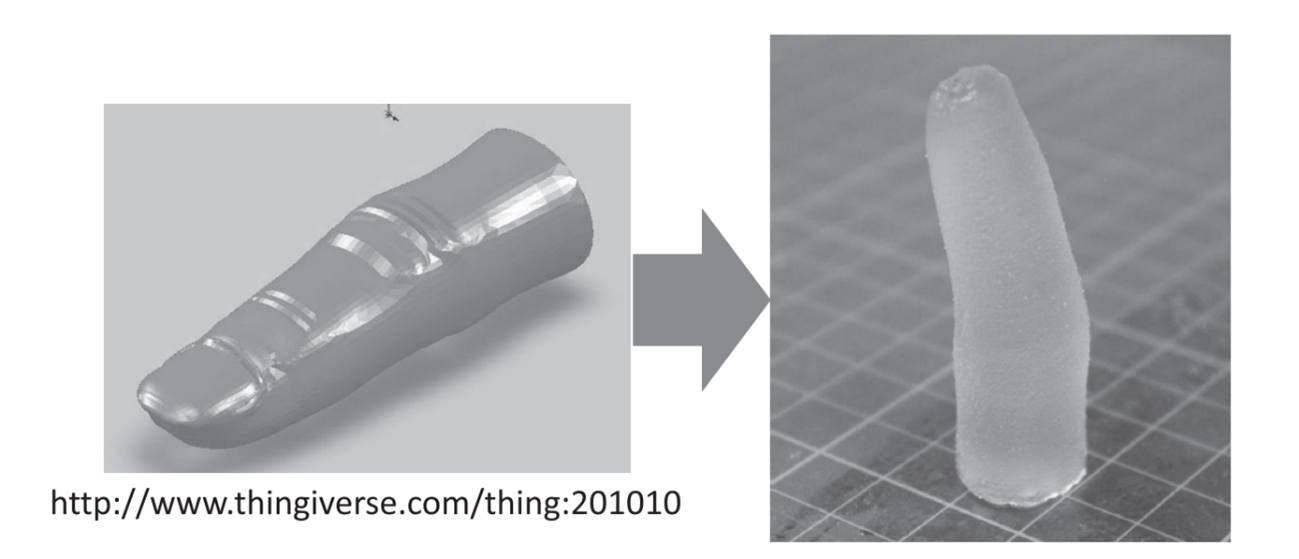
\includegraphics[width=14truecm]{./fig/geru3D.png}
  \caption{3Dゲルプリンターで作製した造形物}
% \url{http://www.this.is.sample.url/} % Web上のデータの場合、参照先URLを明記
  \label{fig:ss}
\end{figure}

これは,ゲル化を誘起するUVレーザーを光ファイバーを通して局所的にゲル溶液に照射することで,ゲルの3次元造形を可能にしている.3Dプリンターは現在,臓器の立体イメージを作り出すのに医療分野で活用されているが,手術の計画や事前検証のための立体の臓器モデルを作製するには,数千万もする工学な3Dプリンターを使用してプラスチックやゴムなどの,実際の臓器よりもはるかに硬い樹脂を用いて造形をする方法しか存在しなかった.
このゲルを用いて印刷する3Dプリンターは,低コストで感触がより患者のものと似ている臓器モデルを作成できる可能性を秘めている.

この3Dプリンターは材料として微粒子調整ダブルネットワークゲル(略称:P-DNゲル)を使用している.このゲルは強電解質性を示すモノマー由来の堅く脆い高分子ネットワーク(1st ネットワーク)と,中性を示すモノマー由来の柔軟な高分子ネットワーク(2nd ネットワーク)が相互侵入網目構造をとっている複合材料である.このP-DNゲル溶液にUVレーザーを照射することでラジカル反応が生じ,ゲルの3次元構造をつくることができる.


\section{Suntory-3D on the Rocks\cite{b}}
\label{sec:enum}

氷を掘削し様々な彫刻を作りお酒に入れて楽しむ試みがある.
多軸の CNC を使い掘削することで高精度の彫刻を作ることができるが,一般に普及させるのはコストならびに加工中の冷却の面から考えると難しい.

\begin{figure}[H]
  \centering
  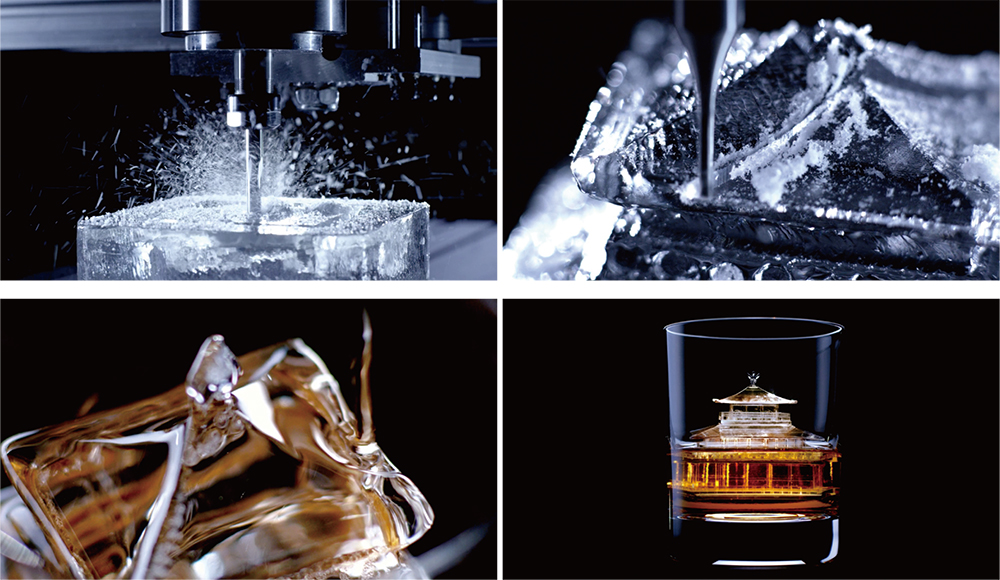
\includegraphics[width=12truecm]{./fig/Suntory.jpg}
  \caption{実際に掘削して作製した高精度の彫刻の例}
  \url{https://mag.sendenkaigi.com/brain/201406/up-to-works/002420.php} % Web上のデータの場合、参照先URLを明記
  \label{fig:Suntory}
\end{figure}


\section{A Layered Fabric 3D Printer for Soft Inter active Objects\cite{c}}
\label{sec:enum}
この研究では布の造形物を印刷するためのプリンターを紹介している.
また,布の中に導電繊維の層を入れたり,コイル状の布を入れることで,タッチセンサーとしての利用法や NFC を使い LED を光らせるアプリケーションが紹介されている.
このプリンターの仕組みは,布のロールを引き出し天板に吸着させ固定し,レーザーでモデルの輪郭を切断し布のロールから切り出す.
この工程を繰り返し,アイロンの熱で接着していくことで造形物が完成する.

\begin{figure}[H]
  \centering
  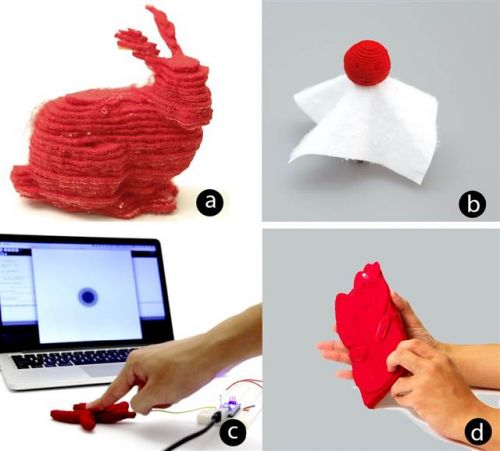
\includegraphics[width=10truecm]{./fig/ALayered.jpg}
  \caption{実際に印刷された布の造形物}
  \url{https://thelastnewspaper.com/a-layered-fabric-3d-printer-for-soft-interactive-objects/} % Web上のデータの場合、参照先URLを明記
  \label{fig:ferret}
\end{figure}



\section{ Additive manufacturing of optically trans-parent glass\cite{d}}
\label{sec:enum}
ガラスをマテリアルに使ったこの研究では,高温で流動性の高い状態に保持されたガラスを貯めておき,そのガラスを垂らすことで造形していく.
実際に造形されたガラスの造形物は一回のストロークで出せるラインは太く分厚いものであり,細かい造形はできないがサイズの大きい花瓶のようなものを造形することができる.
この手法で造形された花瓶は光を乱反射させる特性があり,上からライトを当て光の波紋を楽しむアプリケーションが提示されていた.

\begin{figure}[H]
  \centering
  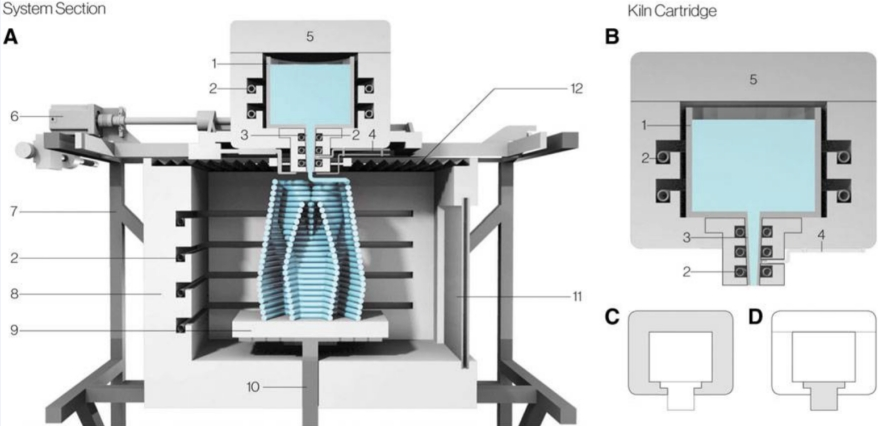
\includegraphics[width=12.5truecm]{./fig/Additive2.jpg}
  \caption{ガラス造形の仕組み}
% \url{http://www.this.is.sample.url/} % Web上のデータの場合、参照先URLを明記
  \label{fig:ferret}
\end{figure}

\begin{figure}[H]
  \centering
  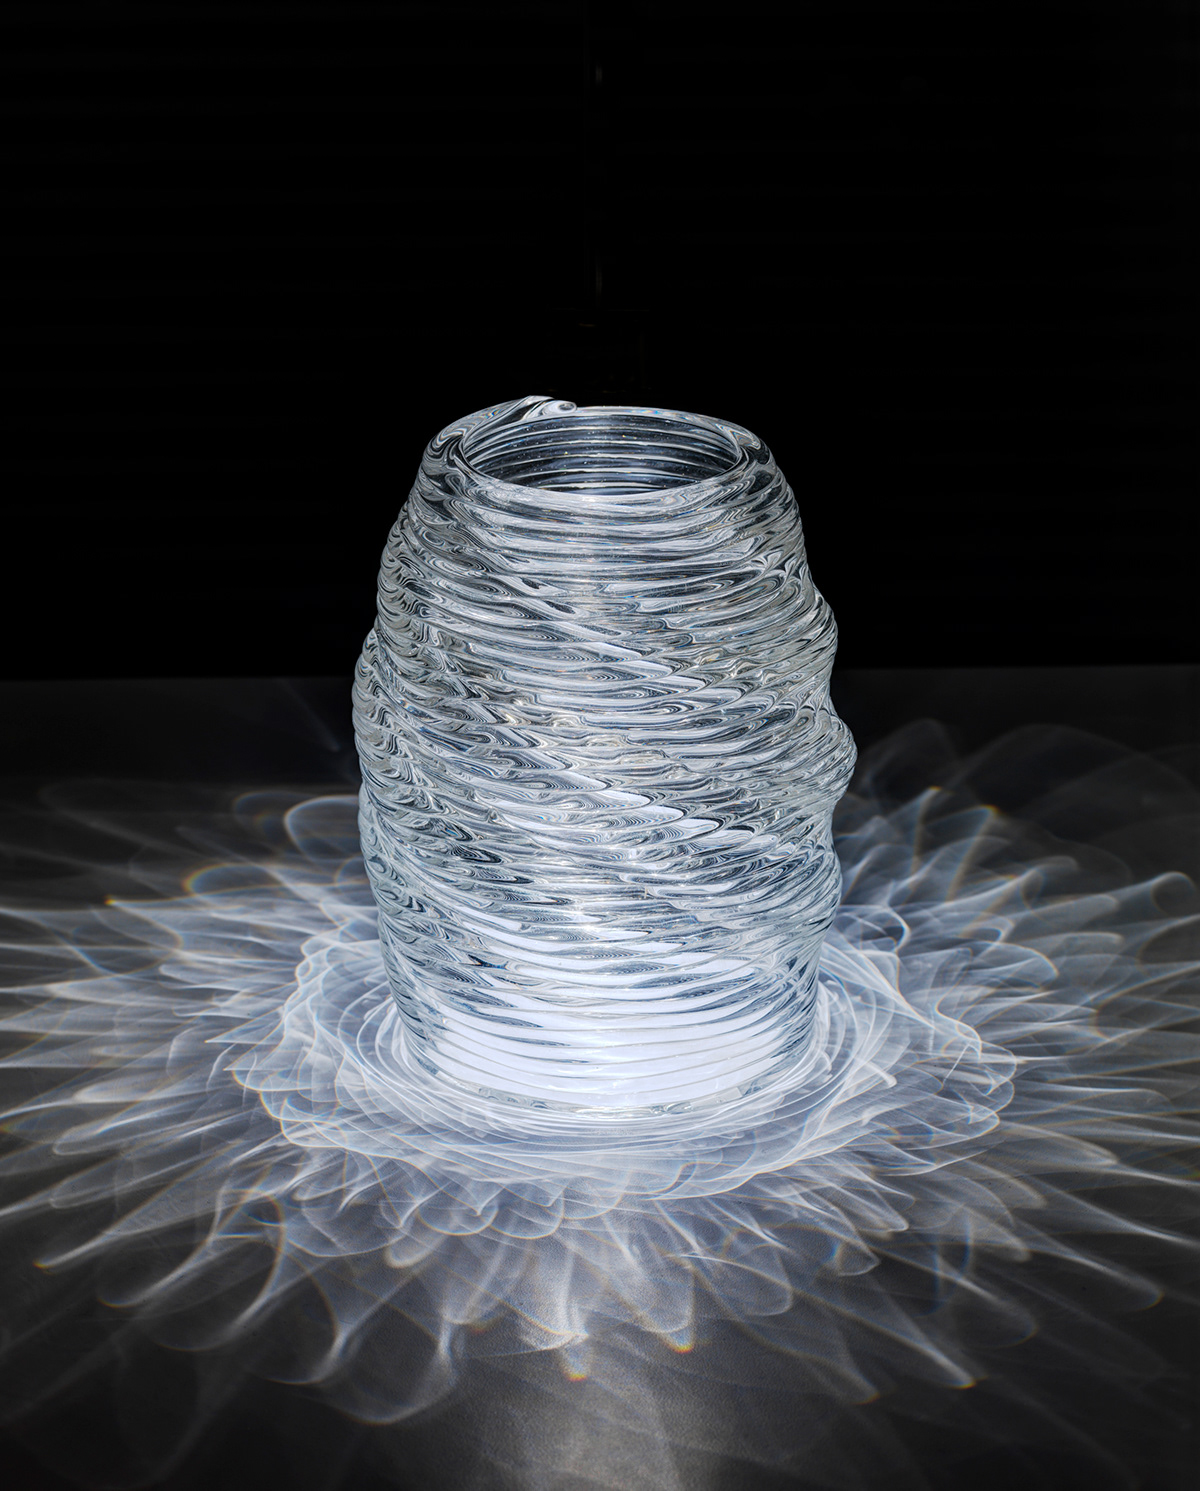
\includegraphics[width=8truecm]{./fig/Additive1.jpg}
  \caption{造形されたガラスの造形物}
  \url{https://www.behance.net/gallery/65276297/GLASS-I} % Web上のデータの場合、参照先URLを明記
  \label{fig:ferret}
\end{figure}

\begin{figure}[H]
  \centering
  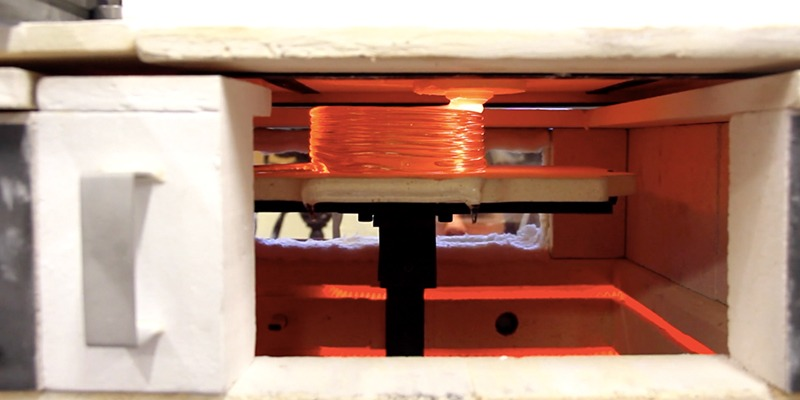
\includegraphics[width=13truecm]{./fig/Additive3.jpg}
  \caption{制作中の様子}
  \url{https://www.solidsmack.com/fabrication/mits-mediated-matter-group-unveils-transparent-glass-3d-printer/} % Web上のデータの場合、参照先URLを明記
  \label{fig:ferret}
\end{figure}


\section{静電インクジェット式3Dプリンタによる高粘度食品材料の高精度プリント\cite{e}}
\label{sec:enum}
この研究では静電インクジェット法を用いることで,高い印刷精度で高粘度材料を用いた,視覚的,味覚的に優れた食品の印刷を可能にする3Dプリンターの開発をしている.

従来の食品の3Dプリンターには熱溶解式(FDM)式3Dプリントを用いたチョコレートの印刷がある.しかし,熱溶解式では積層ピッチが約0.5[mm]以上と非常に粗く,また高粘度材料をプリントする際には添加物を加える必要がある.この添加物には,食品の味に影響が出てくる問題点がある.
静電インクジェット法を用いると,この問題を解決すると同時に高精度な印刷が可能となる.
下の図2.7の様なチョコレートプリンターを作製し,実験を行った.


\begin{figure}[H]
  \centering
  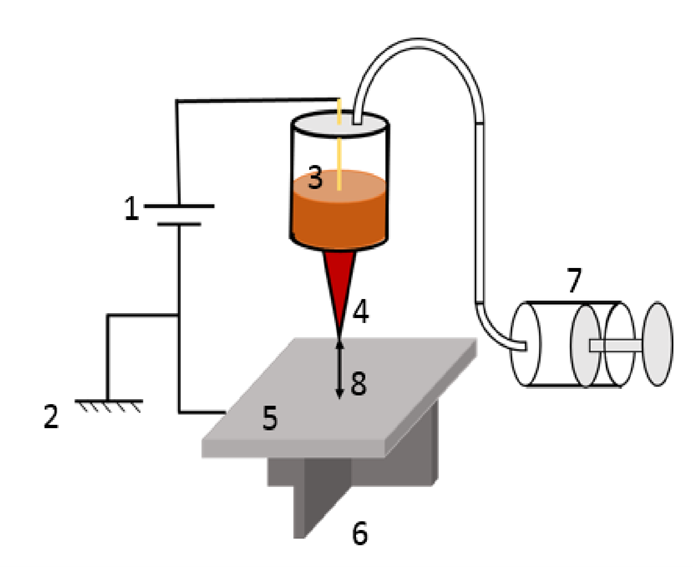
\includegraphics[width=11truecm]{./fig/seidenn.png}
  \caption{静電インクジェット式プリンターによるチョコレートプリントの仕組み}
  %\url{https://thelastnewspaper.com/a-layered-fabric-3d-printer-for-soft-interactive-objects/} % Web上のデータの場合、参照先URLを明記
  \label{fig:ferretss}
\end{figure}

この3Dプリンターは高粘度食品材料であるミルクチョコレートに高電圧を加え微小液滴を吐出し,下図2.8のような超微細なラインを印刷することを可能にする.
また電圧のコントロールによって,吐出するラインの径を制御することもできる.

\begin{figure}[H]
  \centering
  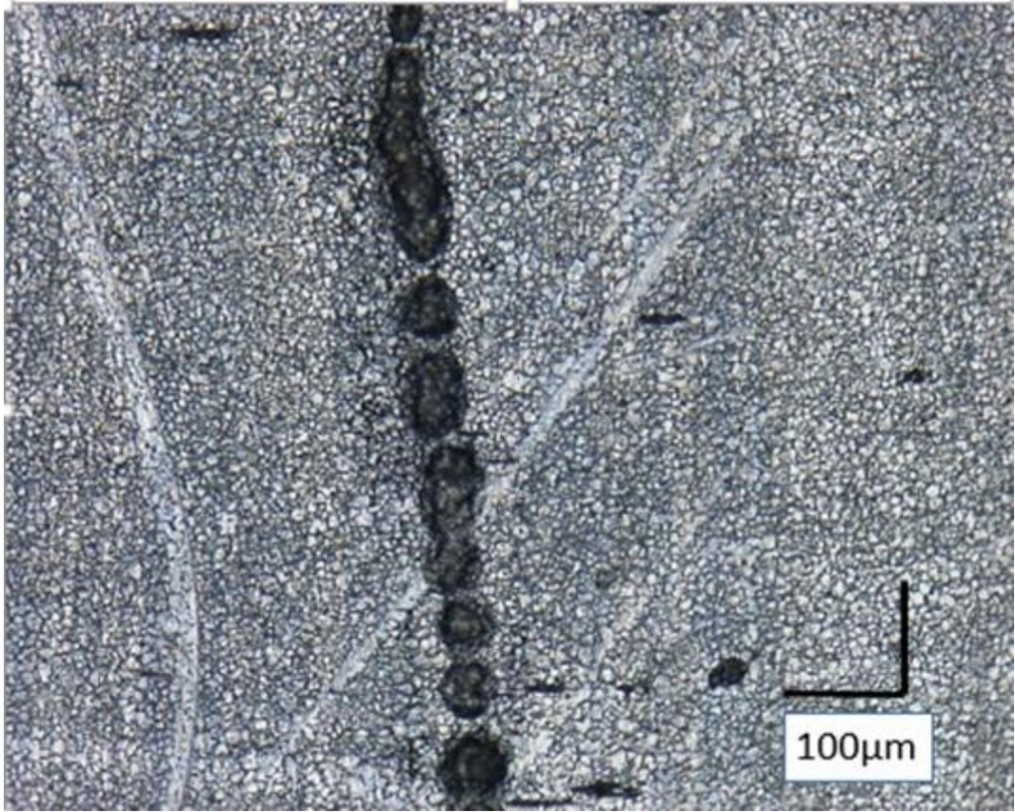
\includegraphics[width=9truecm]{./fig/seidenn2.jpg}
  \caption{実際に吐出されたチョコレートを顕微鏡を用いて観察した様子}
  %\url{https://thelastnewspaper.com/a-layered-fabric-3d-printer-for-soft-interactive-objects/} % Web上のデータの場合、参照先URLを明記
  \label{fig:ferret}
\end{figure}


\section{フルカラー3Dプリンター—2D印刷から3D印刷へ—\cite{f}}
\label{sec:enum}
フルカラー3Dプリンターについて紹介する.
このプリンターはUV(紫外線)硬化インクジェット方式を採用したことで任意の3D形状の造形を可能にすると同時に,その表面にフルカラーで印刷することができる.
このフルカラー3Dプリンターにより,クリエイターの創造物が画面の中だけではなく,今までより容易に手に取れるようになっている.
新しい市場も徐々に出現し始めていて,最近では3D撮影による人文やペットのリアルなコピー造形物が話題になっている.

この3Dプリンターは,下図2.9のようにインクをUV光源で硬化させながら積層法で造形を行う.

\begin{figure}[H]
  \centering
  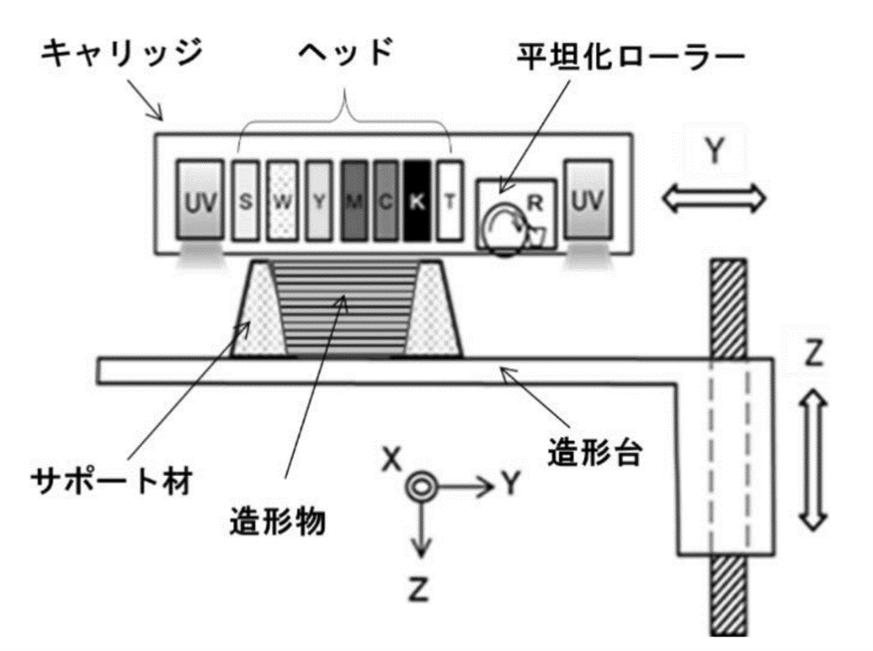
\includegraphics[width=11truecm]{./fig/hurukara.png}
  \caption{フルカラー3Dプリンターの概略図}
  %\url{https://thelastnewspaper.com/a-layered-fabric-3d-printer-for-soft-interactive-objects/} % Web上のデータの場合、参照先URLを明記
  \label{fig:ferret}
\end{figure}

2Dと3Dを比較した時,フルカラー3Dプリンターでは下図2.10のような印刷が行われている.

\begin{figure}[H]
  \centering
  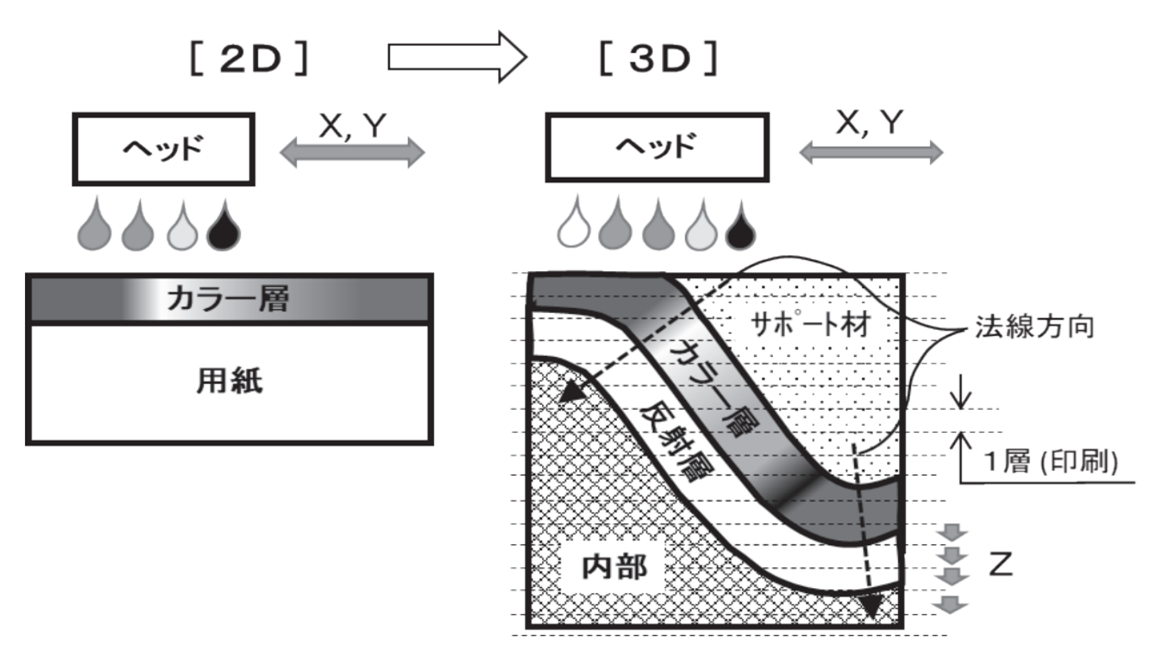
\includegraphics[width=11truecm]{./fig/hurukara2.png}
  \caption{2Dプリンターとフルカラー3Dプリンターの違い}
  %\url{https://thelastnewspaper.com/a-layered-fabric-3d-printer-for-soft-interactive-objects/} % Web上のデータの場合、参照先URLを明記
  \label{fig:ferret}
\end{figure}

2Dの印刷では画像データの濃度によりカラーインクの量が変化するが,これを3Dに適用するとカラー創の外形が崩れてしまうため,カラーインクのない空きスペースには透明インクを補填して外形を保つ工夫をしている.

\section{3D プリンタのセラミックスへの適用\cite{g}}
\label{sec:enum}
この研究では,セラミックス材料を用いた3Dプリンター開発を行っている.
主にセラミックス緻密体を作製する基礎検討に関しての研究である.

今回このプリンタには,SLM方式を採用する.
この方式では下図のように,薄く敷き詰めた粉末床にレーザや電子ビームを走査して粉末を溶解し,順次積層することで3次元の造形物を得る.
昨今では,レーザや電子ビームの出力向上に伴い,新規な材料の適用が可能となってきているが,セラミックスに関しては,急熱急冷を伴うプロセスの特性上衝撃熱が発生するため構造体の密度向上が難しく,工業的な部材の製造は実現していない.
この高密度焼結体の迅速な3次元造形が実現すれば,小ロットの射出成形やテープ整形の代替,複雑形状を生かした高性能セラミックスフィルターや半導体作製用の露光ステージへの利用が期待できる.

\begin{figure}[H]
  \centering
  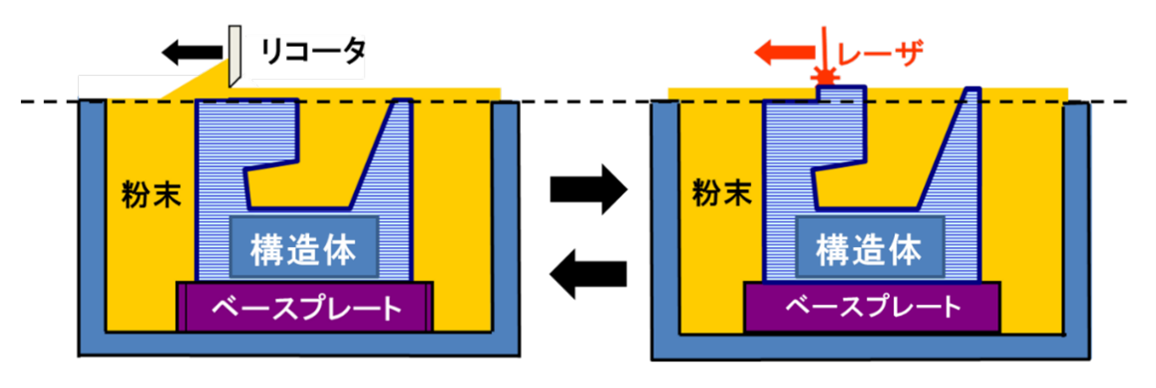
\includegraphics[width=14truecm]{./fig/seramikku1.png}
  \caption{SLM法を用いてセラミックスを印刷する際の様子の模式図}
  %\url{https://thelastnewspaper.com/a-layered-fabric-3d-printer-for-soft-interactive-objects/} % Web上のデータの場合、参照先URLを明記
  \label{fig:ferret}
\end{figure}

熱衝撃を回避したセラミックスのSLM法として,直接セラミックスを焼結せずに,レーザによる形状の作製と焼結による密度向上を分離した間接法が考案されている.この間接法では,セラミックスと低融点の樹脂成分と複合化した粉末を用い,樹脂部分のみをレーザ溶解することでシート成形,グリーン体を作製し,その後,脱脂・焼結することによりセラミックス単体の焼結体を得るものである.間接法を用いた様々な試みがなされてきたが,造形に時間がかかる,密度が低いなどの理由で工業的な利用には未だ至っていない.

この研究では,高強度アルミナ焼結体の作製を目的とした間接法プロセス構築のための検討を行い,アルミナの相対密度が94%の焼結体の作製に成功している.
検討のため,①~③のそれぞれの特性に着目した

①原料セラミックスの選定
・粒子径・粒子径分布

②原料樹脂の選定
・脱脂性・樹脂の融点またはガラス移転点

③造粒粉の作製
・流動性・粒子径・かさ密度・1個粒子の密度

その他にも,SLM条件の最適化,3Dプリンタ内の粉体挙動のシュミレーションを行った結果,以下の図2.12のような,アルミナの相対密度が94%セラミック緻密体を作製することに成功した.

\begin{figure}[H]
  \centering
  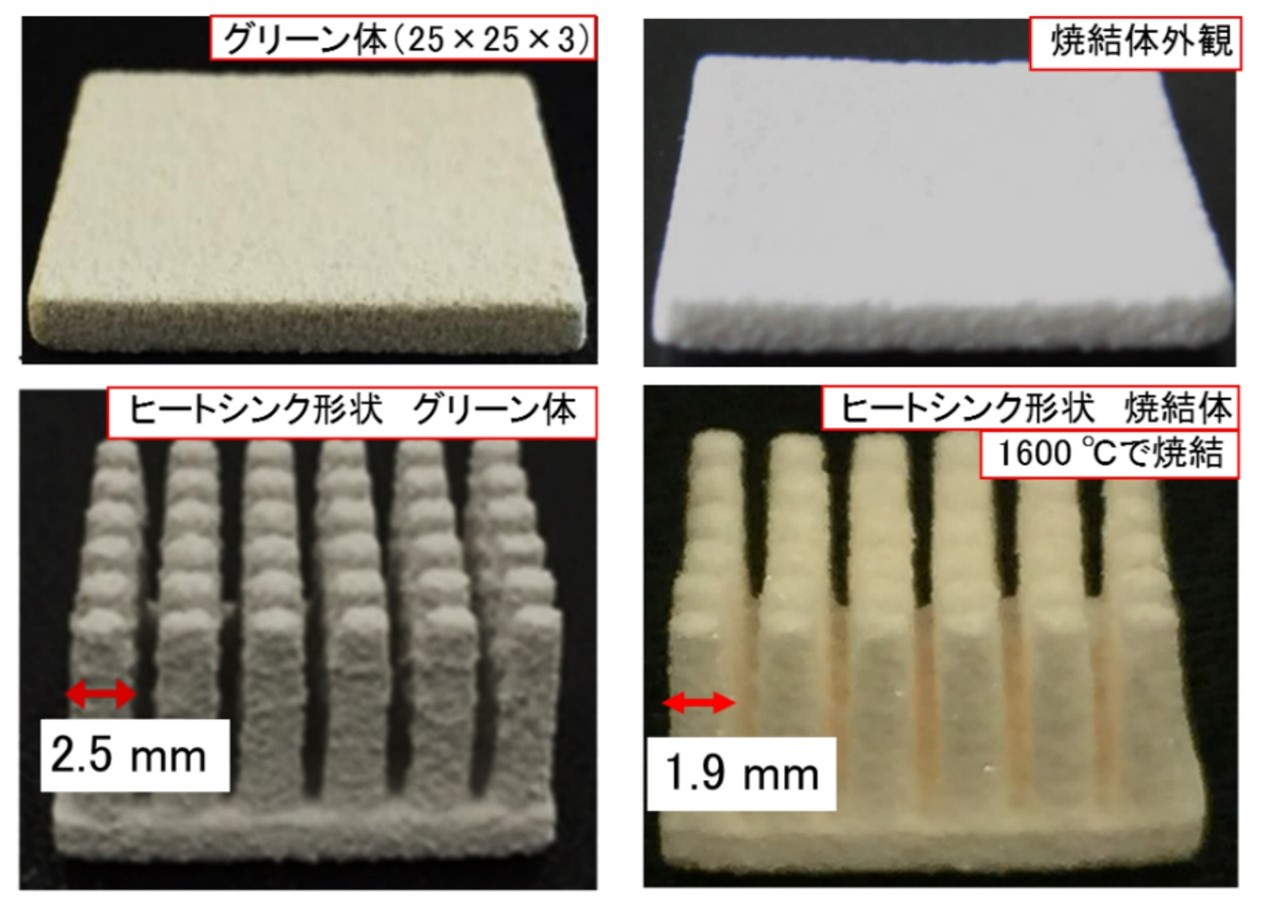
\includegraphics[width=11truecm]{./fig/seramikku.jpg}
  \caption{SLM法を用いた印刷で完成した造形物}
  %\url{https://thelastnewspaper.com/a-layered-fabric-3d-printer-for-soft-interactive-objects/} % Web上のデータの場合、参照先URLを明記
  \label{fig:ferret}
\end{figure}


\section{3D食用ゲルジェットプリンタによる食品創製\cite{i}}
\label{sec:enum}
この研究では,現代の高齢者が食事をより食べやすく,見た目も楽しめるような食品が造形できる,食用のゲルプリンタの開発をしている.

この研究で使用するゲルプリンタは下の概略図のように,①搬送系,②液送系,③冷却系の,三つの機構から成り立っている.

\begin{figure}[H]
  \centering
  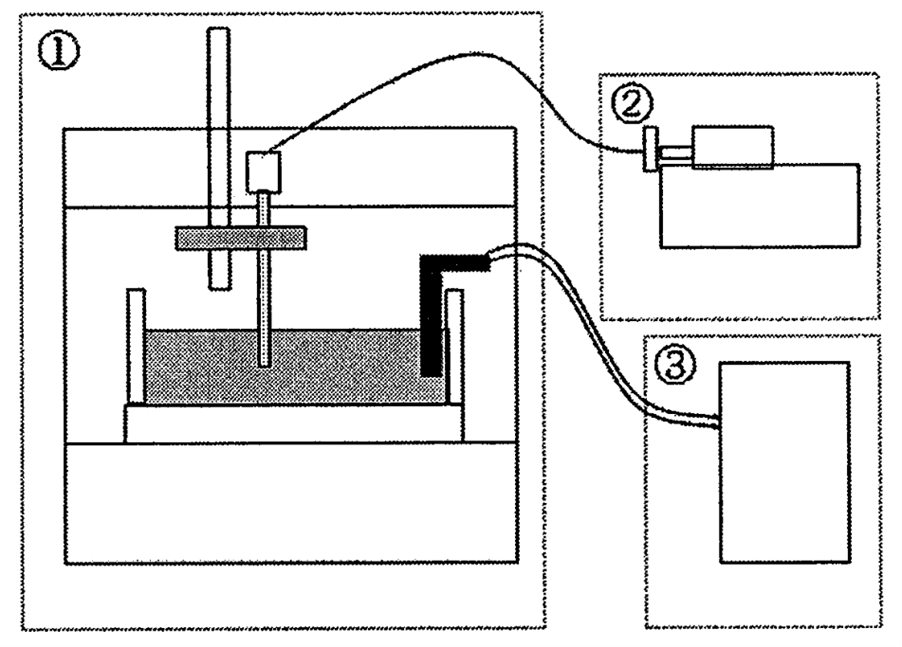
\includegraphics[width=10truecm]{./fig/geru.png}
  \caption{3D食用ゲルジェットプリンタの模式図}
  %\url{https://thelastnewspaper.com/a-layered-fabric-3d-printer-for-soft-interactive-objects/} % Web上のデータの場合、参照先URLを明記
  \label{fig:ferret}
\end{figure}

①は,②のシリンジポンプによって送り出された溶液をコンピュータ制御により,任意の形状に造形することが可能な機構である.②は,ゲルの溶液をシリンジで①の方へ押し出す機構となっている.③は,溶液を滴下する水槽を冷却する機構である.
この装置を用いることで,アルギニン酸ゲル(人工イクラ)の造形が可能となる.

またこの研究では,プリンタに使用するゲルの冷却方法の検討も行った.
寒天とゼラチンの溶液をシリンジを使用しアルミの皿に垂らしていった.1分経過後,寒天,ゼラチン共に固まったが,寒天に比べゼラチンは少し皿にくっついて剝がそうとするとボロボロになった.二つに共通し濃度が高くなると固まりやすくなる傾向があるが,その場合でもゼラチンは強く付着する傾向がある.これは,寒天とゼラチンが植物性と動物性という違いに起因するものだと考えられる.下図が寒天とゼラチンが固まった様子である.

\begin{figure}[H]
  \centering
  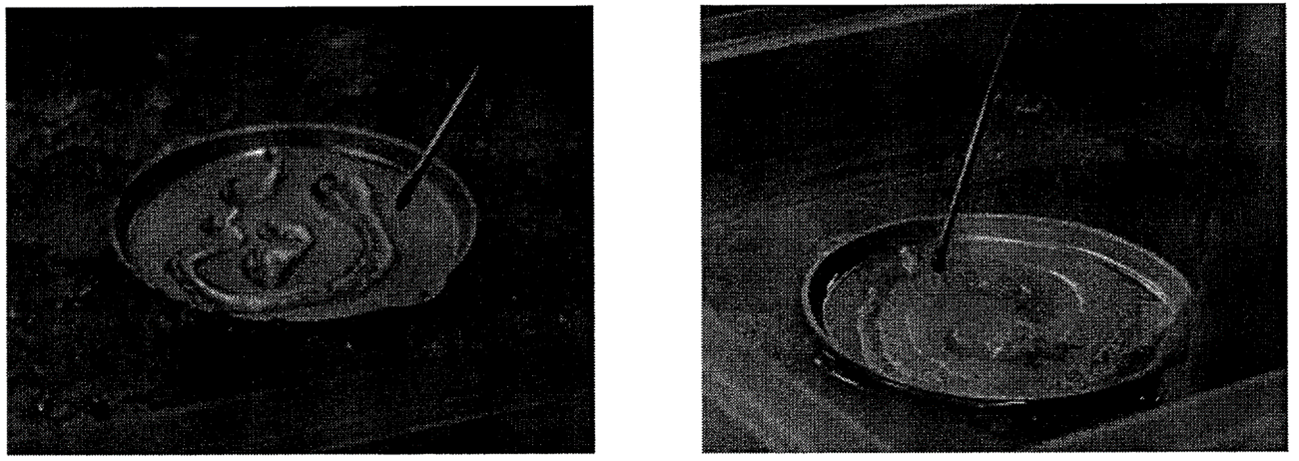
\includegraphics[width=12truecm]{./fig/geru2.png}
  \caption{寒天とゼラチンの溶液をそれぞれアルミの皿に垂らしたときの様子}
  %\url{https://thelastnewspaper.com/a-layered-fabric-3d-printer-for-soft-interactive-objects/} % Web上のデータの場合、参照先URLを明記
  \label{fig:ferret}
\end{figure}

\section{積彩\cite{h}}
\label{sec:enum}
通常の3Dプリンター特にカラー3Dプリンターでも複数の色をせきそうすることでカラー3Dプリンターとしている.
この積彩では,コンピューティングによって調色しながら色糸を積む3Dプリンティングの製造によって造形・着彩をひとつの工程として扱っている.
これを「積彩」と呼び,また,繊細な織物のように糸を積んでいく積彩は新たな表現技法(虹のように変化する色彩効果)を可能にし、この技法を応用して「色瓶」というプロダクト製作している.

\begin{figure}[H]
  \centering
  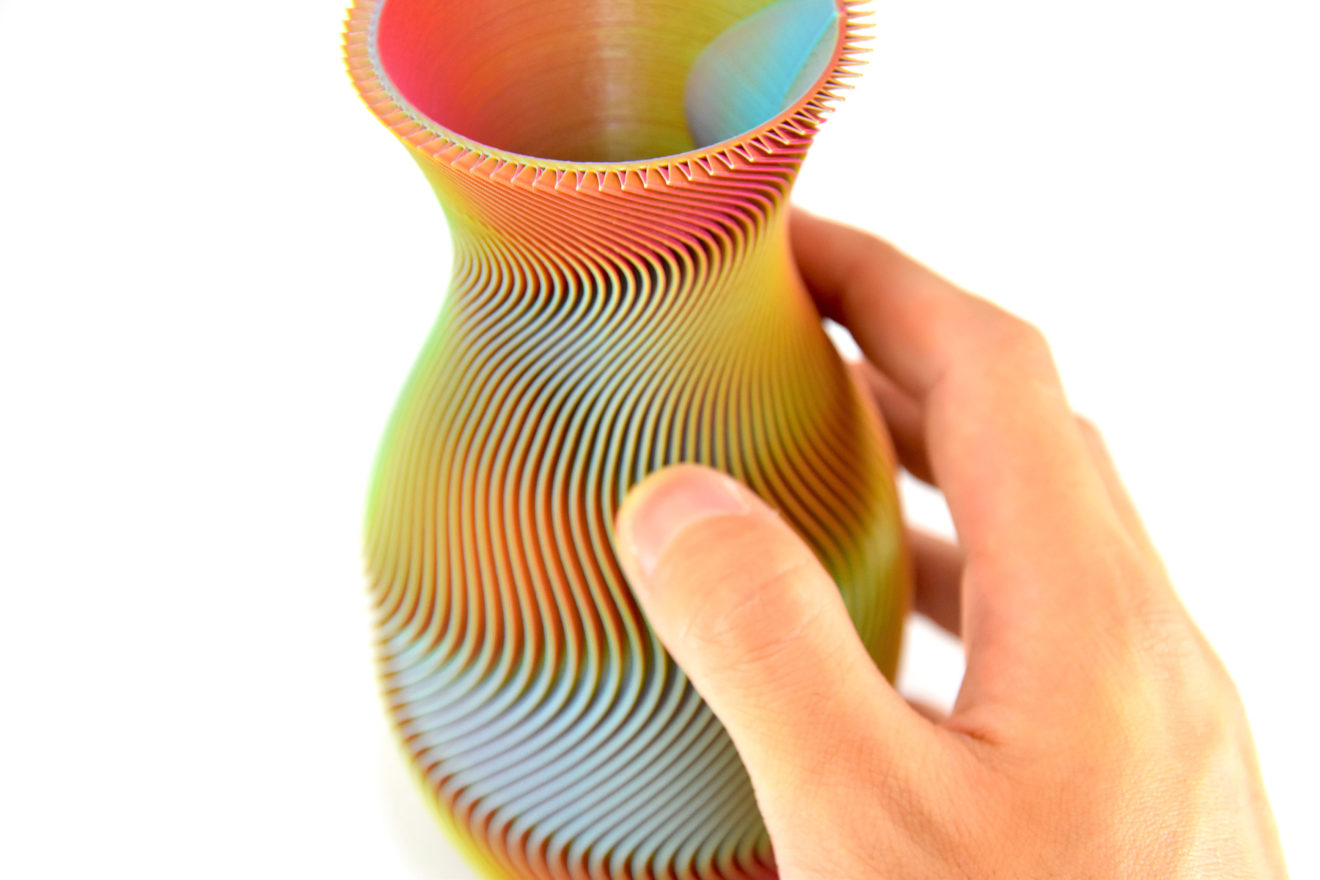
\includegraphics[width=12truecm]{./fig/sekisai.jpg}
  \caption{積彩によって印刷した造形物}
  \url{https://idarts.co.jp/3dp/toyamadesign-gp-color-fab/} % Web上のデータの場合、参照先URLを明記
  \label{fig:ferret}
\end{figure}

\section{放電現象を利用したインクジェット型金属3Dプリンター開発に関する基礎研究\cite{j}}
\label{sec:enum}
この研究では,熱可塑性樹脂を用いた材料押出型の3Dプリンターの機構をベースとした金属3Dプリンターの開発をしている.
従来の金属材料を扱うことのできる3Dプリンターの例として,積層造形,粉末床溶接接合,結合剤噴射,溶接肉盛などを利用したものがあるが,これらの方法は装置も大型で価格も非常に高い.
また,金属粉末の結合力が十分ではない指摘もされている.材料押出型で金属を扱える3Dプリンターが開発されれば,低価格な金属3Dプリンターが実現できる.

下に3Dプリンターの概略図を示す.この3Dプリンターには①細線繰り出し電極,②薄肉パイプ回転電極の二つの特徴がある.

\begin{figure}[H]
  \centering
  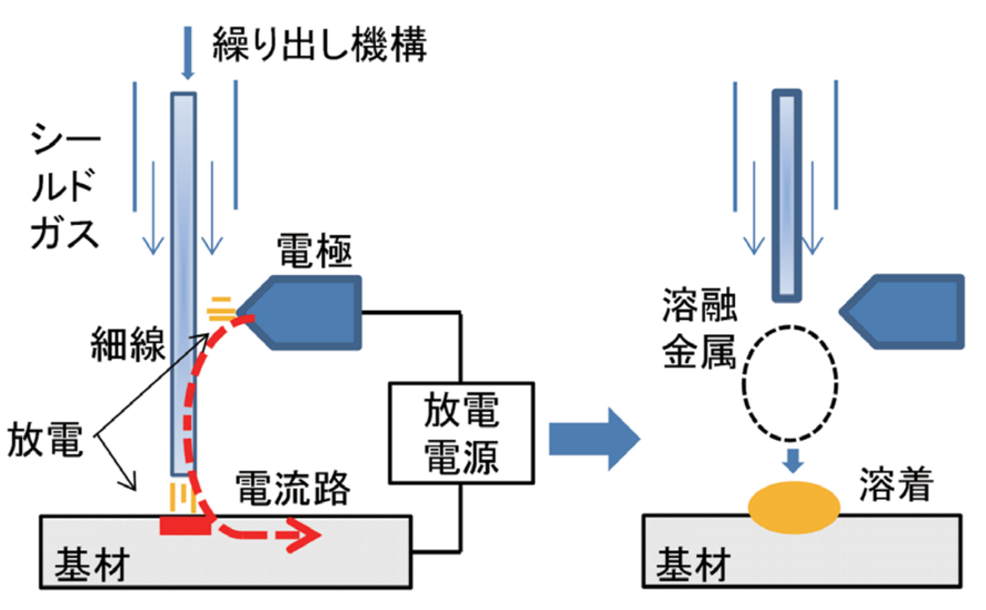
\includegraphics[width=10truecm]{./fig/houdenn.png}
  \caption{インクジェット型金属3Dプリンターの概略図}
  %\url{https://idarts.co.jp/3dp/toyamadesign-gp-color-fab/} % Web上のデータの場合、参照先URLを明記
  \label{fig:ferret}
\end{figure}



\section{高速・高精細金属3Dプリンターの開発\cite{k}}
\label{sec:enum}
この研究では,レーザーメタルでポジションという方法を採用した3Dプリンターの開発を行っている.
この方法はDEDとも呼ばれていて,レーザー粉末を同時に構造物へ照射し,粉末を溶かしながら造形を進める手法であるである以下に印刷している様子の模式図を示す.
レーザーをベースプレートに照射すると融解プールが形成される.金属粉末は,ノズルからキャリアガスとともに噴射され,形成された融解収束される.
供給された粉末は,プールで溶融し,これを冷却することで凝固する.

\begin{figure}[H]
  \centering
  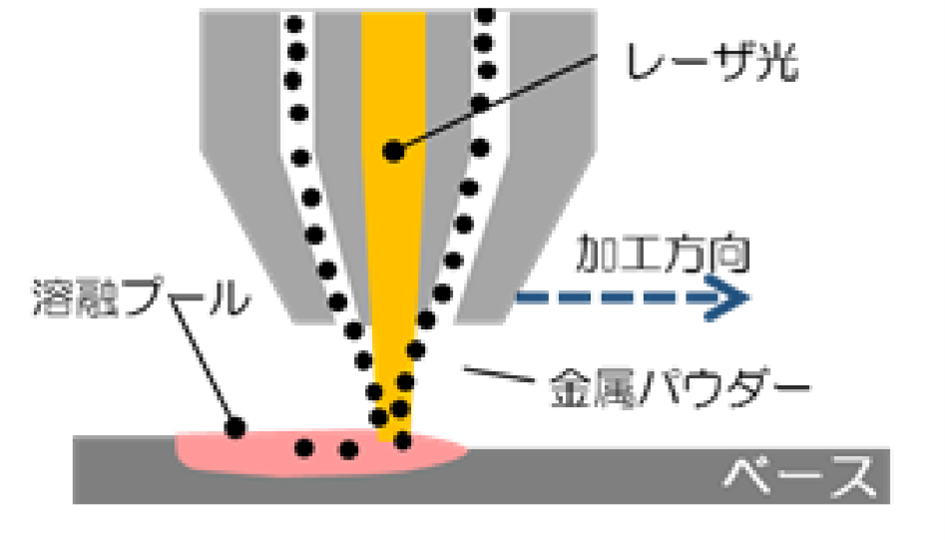
\includegraphics[width=9truecm]{./fig/kinnzoku.png}
  \caption{DEDの模式図}
  %\url{https://idarts.co.jp/3dp/toyamadesign-gp-color-fab/} % Web上のデータの場合、参照先URLを明記
  \label{fig:ferret}
\end{figure}

従来の金属3Dプリンターの多くは,パウダー・ベッド・フュージョン(PB)方式を採用している.
この方式では,パウダーベッドを作製し,造形部のみにレーザーを照射し溶融・凝固スキージとレーザー照射を繰り返して造形を進める.
しかし,高速造形のために高出力レーザーを用いると,パウダーのスパッターが多く発生してしまうという課題がある.
これにたいしDEDは,1.高出力レーザーが使用できるため造形速度が速い,2.局所パージを使用することで筐体レス化が可能となり,大型造形にも対応可能,3.複層造形が可能,などの利点がある.

また,いかにDEDを用いて作製した造形物を示す.
レーザー出力と粉末供給量を増加させることで造形速度が向上し,レーザー出力4kwのときに,最大で359cc/hの造形速度を実現した.

\begin{figure}[H]
  \centering
  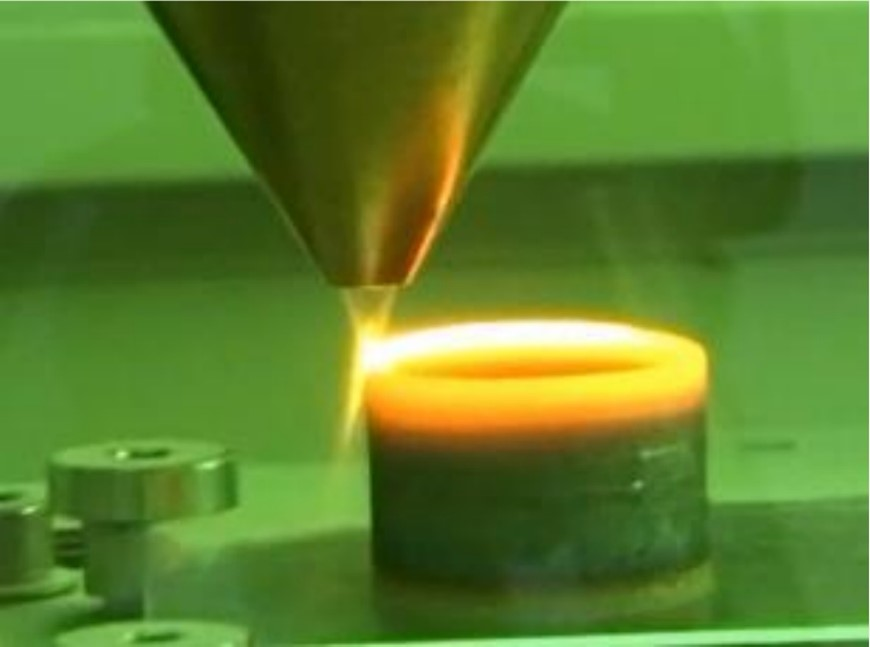
\includegraphics[width=11truecm]{./fig/kinnzoku2.jpg}
  \caption{DEDを用いて作製した造形物}
  %\url{https://idarts.co.jp/3dp/toyamadesign-gp-color-fab/} % Web上のデータの場合、参照先URLを明記
  \label{fig:ferret}
\end{figure}



\section{Robot-Assisted Rapid Prototyping for Ice Structures\cite{ss}}
\label{sec:enum}
この研究では,冷やした水を一滴ずつ垂らしながら氷をFDM の様に積み上げて造形する.
造形のスピードはかなり遅く 20mm/h で造形するが,精密な造形が可能で塩水をサポート剤として使用し,オーバーハングのある造形も可能になっている.
塩水でできた氷は水でできた氷よりも低い温度で溶け始めるため.0℃ の部屋で放置すれば塩水のラフトが溶け水の造形物だけが残る仕組みになっている.
この研究は精度を出すためにスピードを犠牲にしており普通のマグカップのサイズでも印刷に 50 時間近くかかる.
そのため,造形中に溶けないように冷凍庫の中のような環境の部屋で造形する必要がある.


\begin{figure}[H]
  \centering
  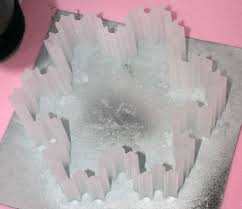
\includegraphics[width=9truecm]{./fig/Robo.png}
  \caption{塩水を使ったラフト}
  %\url{https://idarts.co.jp/3dp/toyamadesign-gp-color-fab/} % Web上のデータの場合、参照先URLを明記
  \label{fig:ferret}
\end{figure}


\section{Elsa:氷を素材とした3d プリンターの開発\cite{h}}
\label{sec:enum}
この研究は造形速度と造形精度を両立させ,一般に普及している3Dプリンターを同じ学習コストで使える氷をマテリアルとした 3D プリンターの開発を行っている.
1つ目の手法として液化した代替フロン (HFC134a) を使用する方法を提案している.
フロンが断熱膨張する際に周囲の熱を奪うのを利用して水を冷やし,瞬時に氷を作る.エアーブラシを使い水とフロンガスを噴射し氷を作る機構を実装した.
しかし,3つの問題点がある.1つ目は,コストが高いことである.3つ目は,造形物がフロンガスを含み純粋な氷ではないこと.3つ目は,環境に対して悪影響があることである.

\begin{figure}[H]
  \centering
  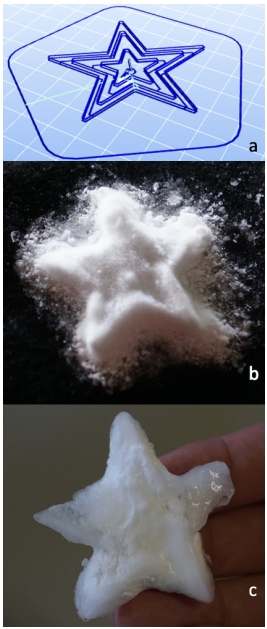
\includegraphics[width=6truecm]{./fig/erusa1.jpg}
  \caption{フロンガスを用いて作製した造形物}
  %\url{https://thelastnewspaper.com/a-layered-fabric-3d-printer-for-soft-interactive-objects/} % Web上のデータの場合、参照先URLを明記
  \label{fig:ferret}
\end{figure}

2つ目の手法として液化した代替フロン (HFC134a) を使用する方法の問題を解決できる氷をマテリアルとした3Dプリンターとして、液体窒素を使用する手法を提案している.

\begin{figure}[H]
  \centering
  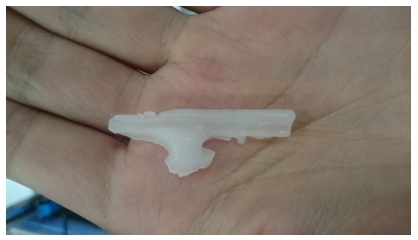
\includegraphics[width=10truecm]{./fig/erusa2.jpg}
  \caption{液体窒素を用いて印刷した造形物}
  %\url{https://thelastnewspaper.com/a-layered-fabric-3d-printer-for-soft-interactive-objects/} % Web上のデータの場合、参照先URLを明記
  \label{fig:ferret}
\end{figure}




